The following block diagram represents a control system that has both feedback and feedforward elements.
\begin{center}
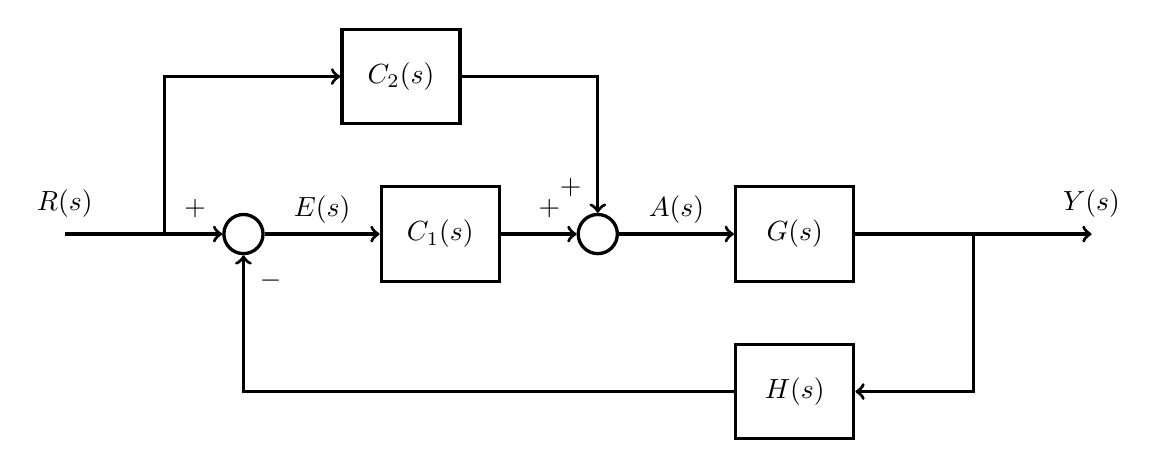
\begin{tikzpicture}[very thick,
sysblock/.style={draw,rectangle,inner sep=6pt,minimum width=1.5cm,minimum height=1.2cm,very thick},
delayblock/.style={draw,rectangle,inner sep=6pt,minimum width=0.5cm,minimum height=1.0cm,very thick},
node/.style={fill,inner sep=0pt,outer sep=0pt},
summer/.style={circle,draw,very thick,inner sep=5pt}]

\draw (-5,0) node[node] (a) {};
\draw (-4,0) node[summer] (sum2) {};
\draw (-2,2) node[sysblock] (C2) {$C_{2}(s)$};
\draw (0.5,0) node[summer] (sum) {};
\draw (3,0) node[sysblock] (G) {$G(s)$};
\draw (-1.5,0) node[sysblock] (C1) {$C_{1}(s)$};
\draw (3,-2) node[sysblock] (H2) {$H(s)$};


\draw[->] (a) |- (C2.180);
\draw[->] (C2.0) -| (sum.90) node[above left=2pt] {$+$};
\draw[<-] (sum2.180) node[above left=2pt] {$+$} -- ++(-2,0) node[above=2pt] {$R(s)$};
\draw[->] (sum2.0) -- node[above] {$E(s)$} (C1.180);
\draw[->] (C1.0) -- (sum.180) node[above left=2pt] {$+$};
\draw[->] (sum.0) -- node[above] {$A(s)$} (G.180);
\draw[->] (G.0) -- ++(3,0) node[above=2pt] {$Y(s)$};
\draw[->] (G.0) -- ++(1.5,0) |- (H2.0);
\draw[->] (H2.180) -| (sum2.-90) node[below right=2pt] {$-$};
\end{tikzpicture}
\end{center}
\begin{enumerate}[(a)]
\item Write down the equations (in terms of $R(s)$, $E(s)$, $A(s)$ and $Y(s)$) that this block diagram represents.
\item  Simplify the block diagram to find $\frac{Y(s)}{R(s)}$.
\end{enumerate}



